\documentclass{beamer}
\usepackage{graphicx}
\usepackage{tikz}
\usepackage{etoolbox}



\documentclass[10pt]{beamer}

% Thème avec bande de couleur en bas
\usetheme{Madrid}
\usecolortheme{seahorse}

\usepackage{etoolbox} % Nécessaire pour les patchs

\makeatletter
\setbeamertemplate{frametitle}{
  \vskip0.3em
  \begin{beamercolorbox}[wd=\paperwidth,ht=2.5ex,dp=1.5ex,leftskip=0.5em,rightskip=1em]{frametitle}
    \usebeamerfont{frametitle}%
    \insertframetitle%
    \hfill
    
\includegraphics[height=1.8ex]{logo_su.png}
  \end{beamercolorbox}
}
\makeatother

\setbeamertemplate{title page}{
  \begin{center}
    \vspace*{2cm}
    \begin{beamercolorbox}[sep=1em,center,wd=0.9\paperwidth,rounded=true,shadow=true]{title}
      {\usebeamerfont{title}\inserttitle\par}
      \vskip1em
      {\usebeamerfont{subtitle}\insertsubtitle\par}
    \end{beamercolorbox}
    \vskip2em
    {\usebeamercolor[fg]{author}\insertauthor\par}
    \vskip1em
    {\usebeamercolor[fg]{institute}\insertinstitute\par}
    \vskip1em
    {\usebeamercolor[fg]{date}\insertdate\par}
  \end{center}
}

\setbeamertemplate{footline}{
  \leavevmode%
  \hbox{%
    \begin{beamercolorbox}[wd=.92\paperwidth,ht=2.5ex,dp=1ex,leftskip=1em, rightskip=1em]{footline}%
      \usebeamerfont{author in head/foot}\insertshortauthor
      \,- 
      \insertshorttitle
    \end{beamercolorbox}%
    \begin{beamercolorbox}[wd=.08\paperwidth,ht=2.5ex,dp=1ex,center]{footline}%
      \insertframenumber{} / \inserttotalframenumber
    \end{beamercolorbox}
  }%
  \vskip0pt%
}

\definecolor{softgreen}{RGB}{80,165,100}


\setbeamercolor{frametitle}{bg=softgreen, fg=white}   
\setbeamercolor{title}{fg=white}                 
\setbeamercolor{author}{fg=black}                  % Auteur
\setbeamercolor{institute}{fg=black}               % Institution
\setbeamercolor{date}{fg=black}                    % Date
\setbeamercolor{footline}{bg=softgreen, fg=white}
\setbeamercolor{footline}{bg=softgreen, fg=white}
\setbeamercolor{section in head/foot}{bg=softgreen, fg=white}
\setbeamercolor{subsection in head/foot}{bg=softgreen, fg=white}
\setbeamercolor{title}{bg=softgreen, fg=white}
\setbeamercolor{subtitle}{fg=white}
\setbeamercolor{block title}{bg=softgreen, fg=white}
\setbeamercolor{block body}{bg=softgreen!10, fg=black}

\setbeamercolor{block title alerted}{bg=red!70, fg=white}
\setbeamercolor{block body alerted}{bg=red!10, fg=black}

\setbeamercolor{block title example}{bg=softgreen!80, fg=white}
\setbeamercolor{block body example}{bg=softgreen!15, fg=black}

% Infos
\title{Projet RITAL - Reproduction de Papier}
\subtitle{On the Benefit of Incorporating External Features in a Neural Architecture for Answer Sentence Selection}
\author{Cai Gautier, Keddis Adam, Théologien Antoine (Les Pupuces)}
\date{\today}

\begin{document}

\begin{frame}
  \titlepage
\end{frame}

\begin{frame}{Sujet du Papier et Contributions Générales}
  \begin{itemize}
    \item \textbf{Sujet principal} : Sélection de réponse (Answer Sentence Selection) dans les systèmes Question/Réponse (QA).
    \item \textbf{Observation clé} : Les architectures neuronales négligent souvent les features externes.
    \item \textbf{Hypothèse} : Les features externes peuvent compléter les réseaux neuronaux.
    \item \textbf{Contribution} : Ajouter des features simples à un réseau convolutionel  (CNN) améliore les performances.
  \end{itemize}
\end{frame}

\begin{frame}{Positionnement par rapport à l'État de l'Art}
  \begin{itemize}
    \item Expérimentation sur deux benchmarks reconnus : \textbf{WikiQA} et \textbf{TRECQA}.
    \item Le Deep Learning domine les approches QA (CNN, LSTM, attention).
    \item Les anciennes features utiles sont souvent ignorées.
    \item L'article explore si elles sont toujours pertinentes.
    \item Comparaison de CNN seul et CNN + features à d'autres modèles de l'état de l'art.
  \end{itemize}
\end{frame}

\begin{frame}{Description du Modèle Proposé}
  \begin{itemize}
    \item \textbf{Architecture CNN} : bi-CNN inspirée de Severyn et Moschitti.
    \item \textbf{Embeddings} : 50D (Wikipedia), 300D (Google News).
    \item \textbf{21 features externes}, en 3 catégories :
    \begin{itemize}
      \item Lexical/semantic matching : BM25, Word2Vec, ESA, TAGME.
      \item Readability : syllabes, mots complexes, Dale-Chall.
      \item Focus : MatchedNGram sur les head words.
    \end{itemize}
    \item \textbf{Fusion} dans la couche fully-connected.
  \end{itemize}
\end{frame}


\begin{frame}{Forces de la Contribution}
  \begin{itemize}
    \item \textbf{Amélioration significative} sur TREC QA et WikiQA.
    \item \textbf{+10.8\% en S@1} sur WikiQA dans certaines configs.
    \item \textbf{Compétitif avec PairwiseRank, ABCNN-3}.
    \item Montre que les CNN seuls ne capturent pas tout.
    \item Soutient l’usage conjoint des features classiques + DL.
  \end{itemize}
\end{frame}

\begin{frame}{Faiblesses et Limitations}
  \begin{itemize}
    \item \textbf{Résultats non systématiquement meilleurs}.
    \item \textbf{Dépendance au dataset/config (dropout, embeddings)}.
    \item \textbf{Features simples}, peu d’analyse approfondie de leur contribution.
    \item \textbf{Portée limitée} à une architecture CNN.
  \end{itemize}
\end{frame}

\begin{frame}{Implémentation - Résultats initiaux}
  \begin{itemize}
    \item Expérimentation via différents paramètres : dropout, mise en place d'un module d'attention, embedding
    \item Dans tous les cas : meilleurs résultats sur \textbf{TRECQA}, sans attention et avec dropout
    \item \textbf{TRECQA} : MAP allant de -3\% à +2.6\%, MRR de -3.8 à +3.5
    \item \textbf{WIKIQA} : MAP allant de -2\% à +7.2\%, MRR de -2.5 à +6.9
  \end{itemize}
\end{frame}

\begin{frame}{Implémentation - Étapes Initiales}
  \begin{itemize}
    \item \textbf{Récupération du code} : Dépôt GitHub fourni par les auteurs.
    \item \textbf{Premier problème} : Deux implémentations distinctes :
    \begin{itemize}
      \item Une version en Python 2.
      \item Une autre en Python 3, mais incomplète.
    \end{itemize}
    \item \textbf{TRECQA} : Dataset déjà formalisé et prêt à l'emploi.
    \item \textbf{WIKIQA} : Format non pris en charge : travail de préparation nécessaire.
  \end{itemize}
\end{frame}

\begin{frame}{Implémentation - Modifications}
  \begin{itemize}
    \item \textbf{Second problème} : Partie du code manquante.
    \begin{itemize}
      \item Génération des identifiants des réponses absente.
    \end{itemize}
    \item \textbf{Notre solution} : Génération via un algorithme simple :
    \begin{itemize}
      \item Utilisation d'un dictionnaire Réponse : Identifiant.
    \end{itemize}
  \end{itemize}
\end{frame}

\begin{frame}{Implémentation - Nos résultats}
 \scriptsize
  \centering
  \begin{tabular}{llc|cc|cc}
    \toprule
    \textbf{System} & \textbf{Attn?} & \textbf{Drop?} & \multicolumn{2}{c|}{\textbf{TREC QA}} & \multicolumn{2}{c}{\textbf{WikiQA}} \\
    & & & MAP & MRR & MAP & MRR \\
    \midrule
    \multicolumn{7}{l}{\textbf{Runs (AQUAINT/Wikipedia)}} \\
    CNN & No & No & 75.25 & 80.90 & \textbf{26.37} & \textbf{26.84}\\
    Combined Model & No & No & \textbf{77.44} & 82.19 & 23.46 & 23.86\\
    Combined Model & No & Yes & \textbf{77.44} & 82.19 & 23.46 & 23.86\\
    CNN & Yes & No & 75.37 & 80.80 & 25.09 & 25.49\\
    Combined Model & Yes & No & 76.59 & 81.45 & 25.23 & 25.66\\
    Combined Model & Yes & Yes & 76.59 & 81.45 & 25.23 & 25.66\\
    \midrule
    \multicolumn{7}{l}{\textbf{Runs (Google News)}} \\
    CNN & No & No & 75.18 & 80.57 & 25.87 & 26.24\\
    Combined Model & No & No & 76.41 & \textbf{82.90} & 24.82 & 25.22\\
    Combined Model & No & Yes & 76.41 & \textbf{82.90} & 24.82 & 25.22\\
    CNN & Yes & No & 74.15 & 80.60 & 25.43 & 25.95\\
    Combined Model & Yes & No & 75.16 & 79.68 & 25.34 & 25.87\\
    Combined Model & Yes & Yes & 75.16 & 79.68 & 25.34 & 25.87\\
    \bottomrule
  \end{tabular}
\end{frame}

\begin{frame}{Implémentation - Evaluation Utilisateur}
  \begin{itemize}
    \item Résultats à relativiser : très petit échantillon
    \item \textbf{Méthode} : Question avec réponses : ordonnancement des réponses
    \item \textbf{Résultat} : \% de bon rang : 0.45 (améliorable)
    \item Le modèle semble bien reconnaître les bonnes et mauvaises réponses mais les ordonne mal
  \end{itemize}
\end{frame}

\begin{frame}{Implémentation - Interprétation}
  \begin{itemize}
    \item L'ajout des features apportent bien des améliorations sur le TREC QA.
    \item Mauvais résultats sur WikiQA : provient sans doute d'une mauvaise reconstruction des données
    \item Couche d'attention moins efficace comme dans le papier original
    \item Dropout qui ne change rien : on a pourtant testé avec différentes valeurs...
  \end{itemize}
\end{frame}

	
	
\begin{frame}{Expérimentations}
    \begin{block}{Comment représenter la sémantique ?}
        \begin{itemize}
            \item LSA ?
            \begin{enumerate}
                \item Réduction de bruit.
                \item Pas de contexte.
                \item Embedding de document.
            \end{enumerate}
            \item Word2vec ?
            \begin{enumerate}
                \item Contextuelle.
                \item Nécessite un grand corpus.
                \item Embedding de mot.
            \end{enumerate}
        \end{itemize}
        
        Finalement, on optera pour un LSA.
    \end{block}
\end{frame}

\begin{frame}{Expérimentations}
    Le LSA réduit les dimensions, donc pour garder cette avantage, on vectorise en token de taille 5 à 7:
    \begin{itemize}
        \item Gestion des mots nouveaux.
        \item Sémantique des "racines".
    \end{itemize}
    On obtient \textbf{1.4M dimensions} au total, puis on applique le LSA pour conserver \textbf{10K dimensions}.\\
    Un document devient donc \underline{la moyenne de ses phrases} (AVG pool).
\end{frame}

\begin{frame}{Expérimentations}
    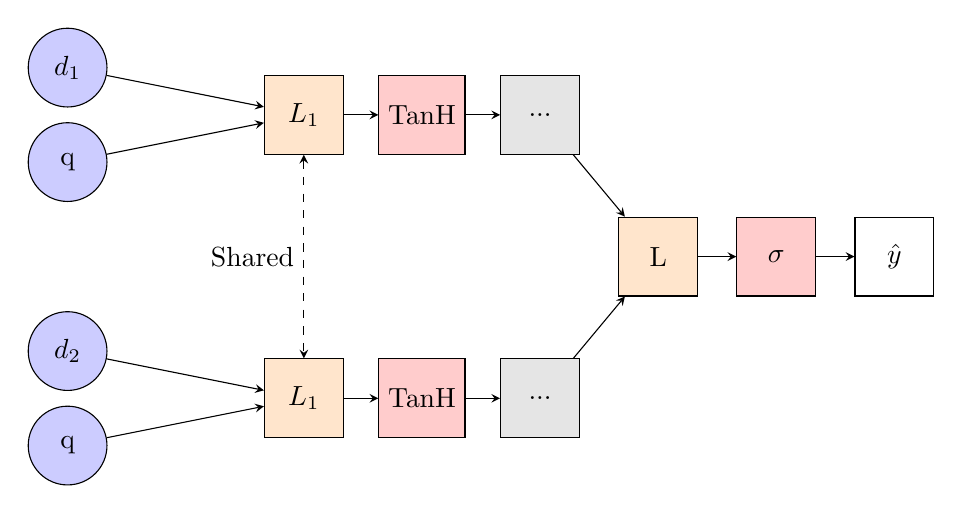
\begin{tikzpicture}[x=1.5cm, y=1.2cm, >=stealth]
        
        \node[circle, draw=black, fill=blue!20, minimum size=1cm] (d1) at (0,-1) {$d_1$};
        \node[circle, draw=black, fill=blue!20, minimum size=1cm] (q1) at (0,-2) {q};
        \node[circle, draw=black, fill=blue!20, minimum size=1cm] (d2) at (0,-4) {$d_2$};
        \node[circle, draw=black, fill=blue!20, minimum size=1cm] (q2) at (0,-5) {q};
        
        \node[rectangle, draw=black, fill=orange!20, minimum size=1cm] (l1) at (2,-1.5) {$L_1$};
        \node[rectangle, draw=black, fill=red!20, minimum size=1cm] (t1) at (3,-1.5) {TanH};
        
        \node[rectangle, draw=black, fill=orange!20, minimum size=1cm] (l2) at (2,-4.5) {$L_1$};
        \node[rectangle, draw=black, fill=red!20, minimum size=1cm] (t2) at (3,-4.5) {TanH};
        
        \node[rectangle, draw=black, fill=gray!20, minimum size=1cm] (p1) at (4,-1.5) {...};
        \node[rectangle, draw=black, fill=gray!20, minimum size=1cm] (p2) at (4,-4.5) {...};
        
        \node[rectangle, draw=black, fill=orange!20, minimum size=1cm] (F) at (5,-3) {L};
        
        \node[rectangle, draw=black, fill=red!20, minimum size=1cm] (S) at (6,-3) {$\sigma$};
        
        \node[rectangle, draw=black, fill=white!20, minimum size=1cm] (Y) at (7,-3) {$\hat{y}$};
        
        \draw[->] (d1) -- (l1);
        \draw[->] (d2) -- (l2);
        
        \draw[->] (q1) -- (l1);
        \draw[->] (q2) -- (l2);
        
        \draw[->] (l1) -- (t1);
        \draw[->] (l2) -- (t2);
        
        \draw[->] (t1) -- (p1);
        \draw[->] (t2) -- (p2);
        
        \draw[->] (p1) -- (F);
        \draw[->] (p2) -- (F);
        
        \draw[->] (F) -- (S);
        
        \draw[->] (S) -- (Y);
        
        \draw[<->, dashed] (l1) -- (l2) node[midway, left] {Shared};
            
    \end{tikzpicture}
    
\end{frame}


\begin{frame}{Expérimentations}
    \begin{block}{Maintenant on "sait" trouver le document, mais la phrase ?}
        \begin{itemize}
            \item Point-wise: Pas d'interactions.
            \item Pair-wise: Intéractions et polyvalent.
            \item List-wise: Encore plus d'interactions 
            mais moins polyvalent.
        \end{itemize}
        
        On opte finalement pour le \textbf{pair-wise} faute de temps/matériel.
        
    \end{block}
\end{frame}

\begin{frame}{Expérimentations}
    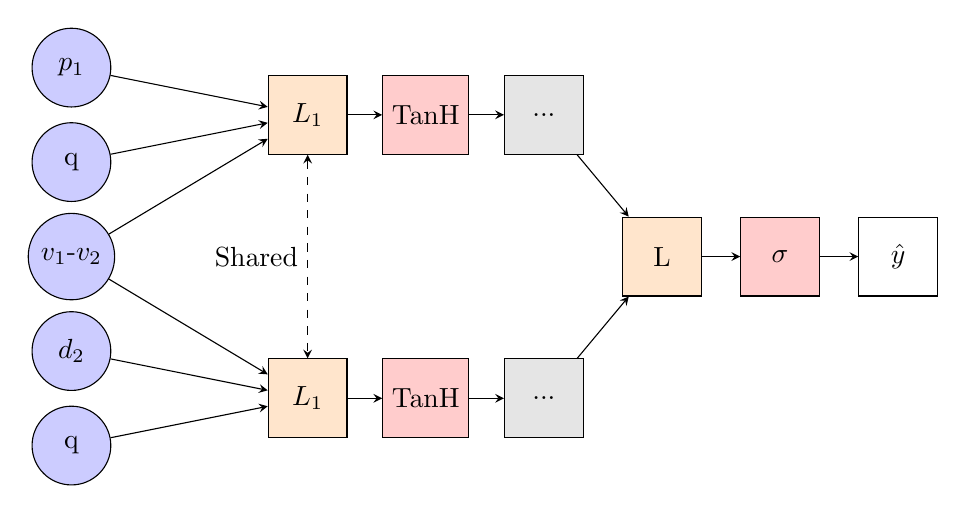
\begin{tikzpicture}[x=1.5cm, y=1.2cm, >=stealth]
        
        \node[circle, draw=black, fill=blue!20, minimum size=1cm] (d1) at (0,-1) {$p_1$};
        \node[circle, draw=black, fill=blue!20, minimum size=1cm] (q1) at (0,-2) {q};
        \node[circle, draw=black, fill=blue!20, minimum size=1cm] (d2) at (0,-4) {$d_2$};
        \node[circle, draw=black, fill=blue!20, minimum size=1cm] (q2) at (0,-5) {q};
        \node[circle, draw=black, fill=blue!20, minimum size=1cm] (v3) at (0,-3) {$v_1$-$v_2$};
        
        \node[rectangle, draw=black, fill=orange!20, minimum size=1cm] (l1) at (2,-1.5) {$L_1$};
        \node[rectangle, draw=black, fill=red!20, minimum size=1cm] (t1) at (3,-1.5) {TanH};
        
        \node[rectangle, draw=black, fill=orange!20, minimum size=1cm] (l2) at (2,-4.5) {$L_1$};
        \node[rectangle, draw=black, fill=red!20, minimum size=1cm] (t2) at (3,-4.5) {TanH};
        
        \node[rectangle, draw=black, fill=gray!20, minimum size=1cm] (p1) at (4,-1.5) {...};
        \node[rectangle, draw=black, fill=gray!20, minimum size=1cm] (p2) at (4,-4.5) {...};
        
        \node[rectangle, draw=black, fill=orange!20, minimum size=1cm] (F) at (5,-3) {L};
        
        \node[rectangle, draw=black, fill=red!20, minimum size=1cm] (S) at (6,-3) {$\sigma$};
        
        \node[rectangle, draw=black, fill=white!20, minimum size=1cm] (Y) at (7,-3) {$\hat{y}$};
        
        \draw[->] (d1) -- (l1);
        \draw[->] (d2) -- (l2);
        
        \draw[->] (v3) -- (l1);
        \draw[->] (v3) -- (l2);
        
        \draw[->] (q1) -- (l1);
        \draw[->] (q2) -- (l2);
        
        \draw[->] (l1) -- (t1);
        \draw[->] (l2) -- (t2);
        
        \draw[->] (t1) -- (p1);
        \draw[->] (t2) -- (p2);
        
        \draw[->] (p1) -- (F);
        \draw[->] (p2) -- (F);
        
        \draw[->] (F) -- (S);
        
        \draw[->] (S) -- (Y);
        
        \draw[<->, dashed] (l1) -- (l2) node[midway, left] {Shared};
        
    \end{tikzpicture}
    
\end{frame}

\begin{frame}{Expérimentations}
    \begin{block}{Qu'est ce que $v_i$ ?}
        On s'inspire de l'article ...
        \begin{itemize}
            \item Length
            \item ExactMatch
            \item Alignement max.
            \item ...
            \item Similarité Cosinus.
        \end{itemize}
        
        Finalement, $v_i \in \mathbb{R}^{17}$, l'idée est que $v_i$ - $v_j$ puisse encoder le plus proche de la query.
    \end{block}
\end{frame}

\begin{frame}{Expérimentations}
    \begin{columns}
        
        \begin{column}{0.48\textwidth}
            \begin{block}{One vs One (document)}
                \begin{itemize}
                    \item Accuracy: 67.02\%
                    \item F1: 0.56
                \end{itemize}
            \end{block}
        \end{column}
        
        \begin{column}{0.48\textwidth}
            \begin{block}{One vs One (phrase)}
                \begin{itemize}
                    \item MRR : 14.89
                    \item MAP : 11.37
                \end{itemize}
            \end{block}
        \end{column}
        
    \end{columns}
\end{frame}

\begin{frame}{Expérimentations}
    \begin{block}{Quelle feature et quel impact ?}
        En mettant simplement les deux features à 0, donc la soustraction n'apportera aucune information, on peut déduire quelle feature a de l'importance dans la prédiction ...\newline
        
        Sans surprise:
        
        \begin{itemize}
            \item ExactMatch : MRR $\pm$1.23
            \item Alignement max: MRR $\pm$0.56
        \end{itemize}
        
    \end{block}
\end{frame}

\begin{frame}{Expérimentations}
    \begin{block}{Les améliorations:}
        
        \begin{itemize}
            \item Vers un modèle \textit{end-to-end}.
            \item Embedding des mots.
            \item List-Wise, donc un réseau par document ?
        \end{itemize}
        
    \end{block}
\end{frame}
    

\begin{frame}{Conclusion}
    
    \begin{itemize}
        \item Veille scientifique.
        \item Ré implémenter des articles.
        \item Essayer des hypothèses.
    \end{itemize}
\end{frame}

\begin{frame}{}
    \centering
    {\Huge Merci pour votre attention ! \newline\newline\newline (Et le semestre)}
\end{frame}

\end{document}
